\documentclass[11pt,letterpaper,twoside]{report}

% Layout
\usepackage{geometry}
\usepackage{setspace}
\usepackage{titlesec}
\usepackage{tocloft}
\usepackage[hang,flushmargin]{footmisc}

% Citation style
\usepackage{harvard}

% Figures
\usepackage{graphicx}
\usepackage{grffile}
\usepackage{subcaption}
\usepackage{epsfig}
\usepackage{multicol}
\usepackage{listings}

% Tables
\usepackage{booktabs}
\usepackage{dcolumn}
\usepackage{multirow}
\usepackage{hhline}
\usepackage{stackengine}
\usepackage{tablefootnote}

% Algorithms
\usepackage[boxed,longend]{algorithm2e}

% Math
\usepackage{amsmath}
\usepackage{amssymb}

% Typography
\usepackage{times}
\usepackage{microtype}
\usepackage{textcomp}

% Macro support
\usepackage{xspace}
\usepackage{color}
\usepackage{ntheorem}

% Diagrams
\usepackage{pgf}
\usepackage{tikz} % extensive form game trees
\usetikzlibrary{calc} % calculating TikZ coordinates
\usetikzlibrary{arrows.meta} % arrows for theory diagrams
\usetikzlibrary{trees}

% PDF links
\usepackage[hidelinks]{hyperref} % backref=page

% Use proper margins.
\geometry{letterpaper,left=1.25in,top=1in,right=1.25in,bottom=1in,nohead}

% double-space text
\doublespacing

% Center chapter titles
% Place chapter title, number, and name on same line
% Make chapter headings all uppercase, standard font size
% Omit page numbers
\titleformat{\chapter}[hang]{\normalfont\fillast\bfseries}{\MakeUppercase{\chaptertitlename} \thechapter: }{0em}{\MakeUppercase}[\thispagestyle{empty}]

% Make section headings normal font size, bold
\titleformat*{\section}{\normalfont\bfseries}
\titleformat*{\subsection}{\normalfont\bfseries}
\titleformat*{\subsubsection}{\normalfont\bfseries}

% Extend to 2in top margins for chapter headings
\titlespacing{\chapter}{0in}{0.62in}{11pt}

% Indent paragraphs four spaces throughout the thesis/dissertation.
\setlength{\parindent}{4ex}

% Tweak spacing of paragraph labels.
\titlespacing{\paragraph}{0in}{0.08in}{0.07in}

% We want numbered subsubsections
\setcounter{secnumdepth}{3}
\setcounter{tocdepth}{3}

% We need to double-space between footnotes.
\setlength{\footnotesep}{13pt}

% Footnotes only one point smaller than text
\renewcommand{\footnotesize}{\small}

% We don't want crazy vertical spacing.
\raggedbottom

% We don't want abandoned words.
\clubpenalty=10000
\widowpenalty=10000

% Prevent awkward hyphenations.
\hyphenation{Raj-kumar}

%% Flush words right at end of paragraph.
%% From: http://tex.stackexchange.com/questions/16330/hfill-after-linebreak
\newcommand\rightparend[1]{{%
      \unskip\nobreak\hfil\penalty50
      \hskip2em\hbox{}\nobreak\hfil\textbf{#1}%
      \parfillskip=0pt \finalhyphendemerits=0 \par}}

% Indented hypothesis environment, subhypotheses
\theoremindent1\parindent
\newtheorem{hyp}{Hypothesis}
\newtheorem{prop}{Proposition}
\makeatletter
\newcounter{subhyp}
\let\savedc@hyp\c@hyp
\newenvironment{subhyp}
{%
	\setcounter{subhyp}{0}%
	\stepcounter{hyp}%
	\edef\saved@hyp{\thehyp}% Save the current value of hyp
	\let\c@hyp\c@subhyp     % Now hyp is subhyp
	\renewcommand{\thehyp}{\saved@hyp\alph{hyp}}%
}
{}
\newcommand{\normhyp}{%
	\let\c@hyp\savedc@hyp % revert to the old one
	\renewcommand\thehyp{\arabic{hyp}}%
}
\makeatother

% Use for commenting
\newcommand{\aak}[1]{{\textcolor{blue}{\textsc{\textbf{[#1 --YN]}}}}}

\begin{document}

% Title page, TOC, etc.
% front matter pages use 2in top margin
\newgeometry{left=1.25in,top=2in,right=1.25in,bottom=1in,nohead}
\pagenumbering{roman}

%1. Title Page
\begin{titlepage}
\begin{center}

% 1. The title of the thesis/dissertation, centered 2� below the top of the page

\vspace{2in}
\begin{singlespace}
\bf
Toward Efficient and Realizable Virtualization of Compute Accelerators
\end{singlespace}


% 2. Your name, centered 1� below the title.
\vspace{61pt} % 1 in = 72pt, 11pt for the line with text
\large Amogh Akshintala
\end{center}


%3. The following statement, within the full mar- gins, 1� below your name:
%�A dissertation [or thesis] submitted to the faculty of the University of North Carolina at Chapel Hill in partial fulfillment of the requirements for the degree of	in the Department [or School or Curriculum] of      .�

\vspace{50pt}
\begin{singlespace}
\noindent \large
A dissertation submitted to the faculty of the University of North Carolina at Chapel Hill
in partial fulfillment of the requirements for the degree of Doctor of Philosophy in
the Department of Computer Science.
\end{singlespace}


%4. On the lower half of the page, centered, the words �Chapel Hill�
%and one line below that, the year in which your committee approves
%the completed thesis/dissertation.
\vspace{50pt}
\begin{center}
\begin{singlespace} \large
Chapel Hill\\
2020
\end{singlespace}
\end{center}

%5. On the right-hand side of the page, �Approved by,� followed by lines for the
%signatures of the adviser and four (two for thesis) readers. List

\vfill
\begin{flushright}
\begin{minipage}[t]{1.8in} \large
Approved by:\\
Michael Ferdman \\
Kevin Jeffay \\
Fabian N. Monrose  \\
Donald E. Porter \\
Christopher J. Rossbach
\end{minipage}
\end{flushright}

\end{titlepage}

%2. Copyright Page (optional)
\newgeometry{left=1.25in,top=8.33in,right=1.25in,bottom=1in,nohead}

%If you wish to copyright your thesis, you must include a copyright page with the following information single-spaced and centered on the bottom half of the page:
%� Year 
%Full Name (exactly as it appears on the title page) 
%ALL RIGHTS RESERVED
%This page should immediately follow the title page, and should bear the lower case Roman numeral: ii.

\begin{center}
\begin{singlespace}
\copyright 2020\\
Amogh Akshintala \\
ALL RIGHTS RESERVED
\end{singlespace}
\end{center}

\clearpage

\newgeometry{left=1.25in,top=2in,right=1.25in,bottom=1in,nohead}

% Normal pages from here on out; TOC title takes care of 2in requirement.
\restoregeometry

%3. Abstract
%The word Abstract should be centered 2? below the top of the page.
%Skip one line, then center your name followed by the title of the
%thesis/dissertation. Use as many lines as necessary. Centered below the
%title include the phrase, in parentheses, (Under the direction of
%_________) and include the name(s) of the dissertation advisor(s).
%Skip one line and begin the content of the abstract. It should be
%double-spaced and conform to margin guidelines. An abstract should not
%exceed 150 words for a thesis and 350 words for a dissertation. The
%latter is a requirement of both the Graduate School and UMI's
%Dissertation Abstracts International.
%Because your dissertation abstract will be published, please prepare and
%proofread it carefully. Print all symbols and foreign words clearly and
%accurately to avoid errors or delays. Make sure that the title given at
%the top of the abstract has the same wording as the title shown on your
%title page. Avoid mathematical formulas, diagrams, and other
%illustrative materials, and only offer the briefest possible description
%of your thesis/dissertation and a concise summary of its conclusions. Do
%not include lengthy explanations and opinions.
%The abstract should bear the lower case Roman number ii (if you did not
%include a copyright page) or iii (if you include a copyright page).

\begin{center}
\vspace*{52pt}
{\normalfont\textbf{ABSTRACT}}
\vspace{11pt}

\begin{singlespace}
Amogh Akshintala: Toward Efficient and Realizable Virtualization of Compute Accelerators \\
(Under the direction of Donald E. Porter, and Christopher J. Rossbach)
\end{singlespace}
\end{center}

The proposed dissertation will focus on developer effort and compatibility in
software virtualization of CPU ISAs, and software virtualization of
specialized compute devices (e.g., GPUs, TPUs) that are programmed through an
API.

Although binary translation is a well-established software ISA virtualization
technique, given the size and complexity of today's dominant ISAs, developers
are routinely forced to adopt ad-hoc techniques to prioritize development
effort. The proposed dissertation will present a principled approach to
determine priority among different parts of the ISA. We believe this data will
be useful to designers of virtual ISAs as well.

Specialized compute accelerators, such as GPUs and TPUs, are usually
controlled through a user-space API.
The proposed dissertation will show that unlike with CPUs, where the ISA is
the canonical interface provided to the programmer, ISA virtualization is
untenable for specialized compute accelerators. Further, the proposed
dissertation will present a present a novel taxonomy, \emph{IEMTS} for cleanly
understanding the design space for virtualizing compute accelerators.
Based on insights from this taxonomy, the proposed dissertation will
present a novel virtualization technique, \emph{hypervisor-mediated
API-remoting}, that is at once realizable and performant.

\clearpage


%4. Dedication, Acknowledgement(s) and/or Preface (all optional)

%A dedication is an honorific statement from the author to a person or group to 
%whom the author commends the effort and product of the dissertation. Most 
%dedications are short statements of tribute beginning with �To��. No heading is 
%required on the dedication page. The text of short dedications should be 
%centered between the left and right margins and 2? from the top of the page.

\begin{center}
\vspace*{52pt}
Dedication\ldots
\end{center}

\pagebreak

%Acknowledgements are the author's statement of gratitude to and
%recognition of the people and institutions who helped the author's
%research and writing.

\begin{center}
\vspace*{52pt}
{\normalfont \textbf{ACKNOWLEDGEMENTS}}
\end{center}

Lorem ipsum dolor sit amet, consetetur sadipscing elitr, sed diam nonumy eirmod tempor invidunt ut labore et dolore magna aliquyam erat, sed diam voluptua. At vero eos et accusam et justo duo dolores et ea rebum. Stet clita kasd gubergren, no sea takimata sanctus est Lorem ipsum dolor sit amet. Lorem ipsum dolor sit amet, consetetur sadipscing elitr, sed diam nonumy eirmod tempor invidunt ut labore et dolore magna aliquyam erat, sed diam voluptua. At vero eos et accusam et justo duo dolores et ea rebum. Stet clita kasd gubergren, no sea takimata sanctus est Lorem ipsum dolor sit amet. Lorem ipsum dolor sit amet, consetetur sadipscing elitr, sed diam nonumy eirmod tempor invidunt ut labore et dolore magna aliquyam erat, sed diam voluptua. At vero eos et accusam et justo duo dolores et ea rebum. Stet clita kasd gubergren, no sea takimata sanctus est Lorem ipsum dolor sit amet.   

Duis autem vel eum iriure dolor in hendrerit in vulputate velit esse molestie consequat, vel illum dolore eu feugiat nulla facilisis at vero eros et accumsan et iusto odio dignissim qui blandit praesent luptatum zzril delenit augue duis dolore te feugait nulla facilisi. Lorem ipsum dolor sit amet,

\clearpage

%\input{frontmatter/preface}

%5. Table of Contents, with page references
\renewcommand{\contentsname}{TABLE OF CONTENTS}
\renewcommand{\cfttoctitlefont}{\hfill\normalfont\bfseries}
\renewcommand{\cftaftertoctitle}{\hfill~}
\renewcommand{\cftdotsep}{1.5}
\cftsetrmarg{1.0in}

\setlength{\cftbeforetoctitleskip}{61pt}
\setlength{\cftaftertoctitleskip}{28pt}

% format chapter entries like other entries
\renewcommand{\cftchapfont}{\normalfont}
\renewcommand{\cftchappagefont}{\normalfont}
\renewcommand{\cftchapleader}{\cftdotfill{\cftdotsep}}

\setlength{\cftbeforechapskip}{15pt}
\setlength{\cftbeforesecskip}{10pt}
\setlength{\cftbeforesubsecskip}{10pt}
\setlength{\cftbeforesubsubsecskip}{10pt}

\begin{singlespace}
\tableofcontents
\end{singlespace}


\clearpage


%6. List of Tables, with titles and page references (if applicable)
\renewcommand{\listtablename}{LIST OF TABLES}
\phantomsection
\addcontentsline{toc}{chapter}{LIST OF TABLES}

\setlength{\cftbeforelottitleskip}{-11pt}
\setlength{\cftafterlottitleskip}{22pt}
\renewcommand{\cftlottitlefont}{\hfill\normalfont\bfseries}
\renewcommand{\cftafterlottitle}{\hfill}

\setlength{\cftbeforetabskip}{10pt}

\begin{singlespace}
\listoftables
\end{singlespace}

\clearpage


%7. List of Figures or Illustrations, with titles and page references (if applicable)
\renewcommand{\listfigurename}{LIST OF FIGURES}
\phantomsection
\addcontentsline{toc}{chapter}{LIST OF FIGURES}

\setlength{\cftbeforeloftitleskip}{-11pt}
\setlength{\cftafterloftitleskip}{22pt}
\renewcommand{\cftloftitlefont}{\hfill\normalfont\bfseries}
\renewcommand{\cftafterloftitle}{\hfill}

\setlength{\cftbeforefigskip}{10pt}
\cftsetrmarg{1.0in}

\begin{singlespace}
\listoffigures
\end{singlespace}
\clearpage


%8. List of Abbreviations (if applicable)
\phantomsection
\addcontentsline{toc}{chapter}{LIST OF ABBREVIATIONS}

\begin{center}
{\normalfont \textbf{LIST OF ABBREVIATIONS}}
\end{center}

\newcommand{\Ab}[2]{\noindent  #1 \> #2 \\}
\newcommand{\Abi}[2]{\noindent #1 \hspace{1.5cm} \= #2 \\}

\aak{THIS IS NOT DONE. IGNORE FOR NOW PLEASE}
\begin{tabbing}
% the first one has to Abi
\Abi{DSA}{Domain Specific Architectures}
\Ab{DSL}{Domain Specific Language}
\Ab{I/O}{Input/Output}
\Ab{IPC}{Inter-Process Communication}
\Ab{IPI}{Inter-Processor Interrupt}
\Ab{AvA}{Accelerated Virtualization of Accelerators}
\Ab{AYO}{Add Your Own in alphabetic order\ldots}
\end{tabbing}

\clearpage


%9. List of Symbols (if applicable)

\pagenumbering{arabic}


% -*- fill-column: 85; -*-
%!TEX root = ../dissertation.tex

\section{Introduction}
\label{s:intro}

\begin{figure}[!htp]
	\centering
	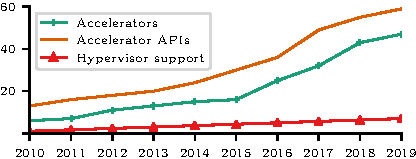
\includegraphics[width=0.7\linewidth]{ava/data/technology_trend/technology_trend.pdf}%
	\caption{The number of accelerators (discrete GPUs and AI
      accelerators) and APIs released since 2010 compared to the number of accelerators officially supported by production hypervisors (VMware ESX, Citrix XenServer, and Microsoft Hyper-V).
      % \ref{l:api_revisions} API major revisions; \ref{l:accelerator_arch} accelerator architectures; \ref{l:hypervisor_arch_support} accelerator architectures supported by hypervisors.
      This data was drawn from release notes and specification sheets.
      % TODO: \amp{This figure has been squished vertically. Regenerate with new aspect-ratio so as to avoid ugly squished text.}
  %\reviewer{F}{I don't think Fig 1 is of much use, your work is a case in point: A single automated approach can deal with many architectures and API revisions, so what is to be read from this?}
  %\cjr{F is pointing out our contribution, but somehow missing it. Dispatched by adding a bullet to the contribution list that claims exactly this.}
  }
	\label{fig:trends}
\end{figure}

Hypervisors have not kept pace with accelerator innovation. Figure~\ref{
fig:trends} shows the evolution of accelerator framework APIs, accelerator
architectures, and hypervisor support for them over the last decade.
Specialized hardware and frameworks emerge far faster than hypervisors support
them and the gap is widening. Many factors contribute to this trend, but lack
of demand is \emph{not} among them, evinced by the wide variety of
accelerators currently available from cloud providers~\cite{amazon_ec2,
google-gpu,google-cmle,gpucloud,amazon_f1,olympus,cloud-tpu}.
The challenge is technical: hypervisor-level accelerator virtualization
requires substantial engineering effort and the design space features multiple
fundamental trade-offs for which a ``sweet spot'' has remained elusive.

Practical virtualization must support sharing and isolation under flexible
policy with minimal overhead. The structure of current accelerator stacks
makes this combination extremely difficult to achieve.
Accelerator stacks are \emph{silos} (Figure~\ref{fig:silo}) comprising
proprietary layers communicating through memory mapped interfaces.
This opaque organization makes it \emph{impractical} to interpose intermediate
layers to form an efficient and compatible virtualization boundary
(\S\ref{s:properties}).
The remaining interposable interfaces leave designers with untenable
alternatives that sacrifice critical virtualization properties such as
interposition and compatibility.

This chapter describes \AvA, which addresses the fundamental limitations of
existing accelerator virtualization techniques.
\AvA combines API-agnostic para-virtual stack components with a DSL
(Domain-Specific Language) and a compiler to automate construction and
deployment of guest libraries, hypervisor-level resource management, and
\workers. \AvA uses an abstract para-virtual device to serve as a transport
endpoint for forwarding the public APIs of vendor-provided frameworks
(e.g. CUDA or TensorFlow). Unlike currently popular user-space API remoting
solutions~\cite{bitfusion,xaas,vmCUDA,rCUDA,cu2rcu}, \AvA preserves hypervisor-level resource management and strong isolation using a novel
technique called \emph{\hirafull (\hira)}.
\hira forwards API calls over hypervisor-managed communication
channels, inserting au\-to\-ma\-tically-generated resource management
components at the transport layer to enforce policies from the DSL
specification. Critically, \emph{automation} from \AvA enables hypervisors
to keep up with fast accelerator evolution: automatic generation of components
dramatically shortens the development cycle. As Figure~\ref{fig:trends}
suggests, a solution that tracks API framework evolution can track hardware
evolution as well.

\AvA supports a broad range of currently-shipping compute offload
accelerators. We virtualized \numaccelerators accelerators including NVIDIA
and AMD GPUs, Google TPUs, and Intel QuickAssist. Virtualizing an API
framework using \AvA requires modest developer effort: a single developer
virtualized OpenCL in a handful of days, a stark contrast to the person-years
of developer effort for VMware's SVGA II~\cite{dowty2009gpu} or BitFusion's
FlexDirect~\cite{bitfusion}. \AvA provides near-native performance
(e.g., 2.4\% slowdown for TensorFlow and 5.6\% for CUDA), enforces isolation
and fair sharing (\S\ref{s:properties}) across guests, and supports live
migration. \AvA is available on GitHub \mbox{\href{https://github.com/utcs-scea/ava}{utcs-scea/ava}}.

% Concretely, this chapter makes the following contributions:

% \begin{itemize}[nosep,leftmargin=1em,labelwidth=*,align=left]
% \item We demonstrate feasibility of automatically constructed virtual accelerator support, using a single technique to support many architectures, APIs, versions, and policies.
% \item We introduce \hirafull (\hira) to enable
% hypervisor-enforced isolation and sharing policies unachievable with current
% SR-IOV and API remoting systems (\S\ref{s:motivation}).
% \item We describe a novel DSL, \Lapis, for describing API functions, resources, and policies to enable automatic construction of virtual stacks starting from native API header files.
% \item We evaluate \AvA on \numaccelerators accelerators showing low effort, strong properties, and good performance (\S\ref{s:eval}).
% \item We identify fundamental challenges in the accelerator virtualization design space (\S\ref{s:background}).
% \end{itemize}


% % Appendices
% \appendix

% % Switch to 1" title margins for appendices
% \titlespacing{\chapter}{0in}{-.38in}{11pt}

% % Appendix 1
% \input{ap1}

% % Appendix 2
% \input{ap2}

% References
\clearpage
\phantomsection

{
\def\chapter*#1{} % suppress bibliograph header.
\begin{singlespace}
\addcontentsline{toc}{chapter}{BIBLIOGRAPHY}
\begin{center}
\normalfont \textbf{BIBLIOGRAPHY}
\vspace{17pt}
\end{center}

\bibliographystyle{plain}
\bibliography{ref}
\end{singlespace}
}

\end{document}